
%% 
%% Copyright 2007, 2008, 2009 Elsevier Ltd
%% 
%% This file is part of the 'Elsarticle Bundle'.
%% ---------------------------------------------
%% 
%% It may be distributed under the conditions of the LaTeX Project Public
%% License, either version 1.2 of this license or (at your option) any
%% later version.  The latest version of this license is in
%%    http://www.latex-project.org/lppl.txt
%% and version 1.2 or later is part of all distributions of LaTeX
%% version 1999/12/01 or later.
%% 
%% The list of all files belonging to the 'Elsarticle Bundle' is
%% given in the file `manifest.txt'.
%% 
%% Template article for Elsevier's document class `elsarticle'
%% with harvard style bibliographic references
%% SP 2008/03/01

\documentclass[preprint,12pt]{elsarticle}

%% Use the option review to obtain double line spacing
%% \documentclass[authoryear,preprint,review,12pt]{elsarticle}

%% Use the options 1p,twocolumn; 3p; 3p,twocolumn; 5p; or 5p,twocolumn
%% for a journal layout:
%% \documentclass[final,1p,times,authoryear]{elsarticle}
%% \documentclass[final,1p,times,twocolumn,authoryear]{elsarticle}
%% \documentclass[final,3p,times,authoryear]{elsarticle}
%% \documentclass[final,3p,times,twocolumn,authoryear]{elsarticle}
%% \documentclass[final,5p,times,authoryear]{elsarticle}
%% \documentclass[final,5p,times,twocolumn,authoryear]{elsarticle}

%% For including figures, graphicx.sty has been loaded in
%% elsarticle.cls. If you prefer to use the old commands
%% please give \usepackage{epsfig}

%% The amssymb package provides various useful mathematical symbols
\usepackage{amsmath,amssymb,bm}
%\usepackage[dvips,colorlinks=true,citecolor=green]{hyperref}
\usepackage[colorlinks=true,citecolor=green]{hyperref}
%% my added packages
\usepackage{verbatim}
\usepackage{caption}
\usepackage{subcaption}
\usepackage{booktabs} % for nice tables
\usepackage{multirow} % for multirows in tables
%\usepackage{breqn}
% matrix command 
\newcommand{\matr}[1]{\mathbf{#1}} % bold upright (Elsevier, Springer)
% vector command 
\newcommand{\vect}[1]{\mathbf{#1}} % bold upright (Elsevier, Springer)
\newcommand{\ud}{\mathrm{d}}
\renewcommand{\vec}[1]{\mathbf{#1}}
\newcommand{\veca}[2]{\mathbf{#1}{#2}}
\renewcommand{\bm}[1]{\mathbf{#1}}
\newcommand{\bs}[1]{\boldsymbol{#1}}
\graphicspath{{figs/}{../../figures/}}
%% The amsthm package provides extended theorem environments
%% \usepackage{amsthm}
%% The lineno packages adds line numbers. Start line numbering with
%% \begin{linenumbers}, end it with \end{linenumbers}. Or switch it on
%% for the whole article with \linenumbers.
%% \usepackage{lineno}
\journal{Composite Structures}
\begin{document}
	\begin{frontmatter}
		%% Title, authors and addresses
		%% use the tnoteref command within \title for footnotes;
		%% use the tnotetext command for theassociated footnote;
		%% use the fnref command within \author or \address for footnotes;
		%% use the fntext command for theassociated footnote;
		%% use the corref command within \author for corresponding author footnotes;
		%% use the cortext command for theassociated footnote;
		%% use the ead command for the email address,
		%% and the form \ead[url] for the home page:
		%% \title{Title\tnoteref{label1}}
		%% \tnotetext[label1]{}
		%% \author{Name\corref{cor1}\fnref{label2}}
		%% \ead{email address}
		%% \ead[url]{home page}
		%% \fntext[label2]{}
		%% \cortext[cor1]{}
		%% \address{Address\fnref{label3}}
		%% \fntext[label3]{}
		
		\title{Elastic constants identification of fibre-reinforced composites by using guided wave dispersion curves and genetic algorithm for improved simulations}
		
		%% use optional labels to link authors explicitly to addresses:
		%% \author[label1,label2]{}
		\address[IFFM]{Institute of Fluid Flow Machinery, Polish Academy of Sciences, Poland}
		
		\author{Pawel Kudela\corref{cor1}\fnref{IFFM}}
		\ead{pk@imp.gda.pl}
		\author{Maciej Radzienski\fnref{IFFM}}
		\author{Piotr Fiborek \fnref{IFFM}}
		%\ead{pfiborek@imp.gda.pl}
		\author{Tomasz Wandowski \fnref{IFFM}}	
		
		\cortext[cor1]{Corresponding author}
		
\begin{abstract}
			%% Text of abstract
There is a great potential for model-based approaches in which guided waves are utilised for damage detection, localisation and size estimation. 
However, to be effective, the model must accurately represent guided wave propagation behaviour, especially wave velocity dependence on the angle of propagation. 
Unfortunately, improperly assumed or derived through homogenisation elastic material properties can lead to larger wave velocity changes than caused by damage. 
In order to account for this problem, the elastic constants are estimated based on experimental measurements of Lamb waves and optimisation techniques. 

In the proposed approach, experimental measurements of full wavefield data of propagating Lamb
waves are conducted by scanning laser Doppler vibrometer. 
The obtained wavefield data is processed by using the 3D Fourier transform. 
Slicing the data at selected frequencies yields wavenumber profiles. 
These profiles can be directly translated to wave propagation velocity dependence on the angle of propagation. 
Data can also be sliced at selected angles giving dispersion curve images. 
At the same time, wavenumber profiles or dispersion curves can be calculated by using a semi-analytical model for the range of material properties. 
A genetic algorithm is used in which the best fit between experimental data and the semi-analytical model is optimised.

Experiments were conducted on a unidirectional CFRP panel and the above-mentioned procedure was applied. 
Identified material properties were used in the in-house code of the time domain spectral element method for simulations of the propagating waves. 
Finally, numerical results were compared to the experimental full wavefield data showing much better accuracy than in case of application of homogenisation techniques.

Furthermore, the correctness of elastic constants determined by the proposed method was validated against the elastic constants obtained through static test standards.
\end{abstract}
		
		\begin{keyword}
			%% keywords here, in the form: keyword \sep keyword
			Lamb waves \sep dispersion curves \sep semi-analytical spectral element method \sep composite laminates \sep elastic constants.
			%% PACS codes here, in the form: \PACS code \sep code
			
			%% MSC codes here, in the form: \MSC code \sep code
			%% or \MSC[2008] code \sep code (2000 is the default)
			
		\end{keyword}
		
	\end{frontmatter}
	
	%% \linenumbers
	
	%% main text
%%%%%%%%%%%%%%%%%%%%%%%%%%%%%%%%%%%%%%%%%%%%%%%%%%%%%%%%%%%%%%%%%%%%%%%%%%%%%%%%
\section{Introduction}
%%%%%%%%%%%%%%%%%%%%%%%%%%%%%%%%%%%%%%%%%%%%%%%%%%%%%%%%%%%%%%%%%%%%%%%%%%%%%%%%
Composite laminates such as carbon fibre-reinforced polymers (CFRP) have found a wide range of applications in the aerospace, automotive and energy industries as well as in everyday products. Knowledge about their mechanical properties is indispensable for the modelling and design purposes.
However, elastic constants representing material properties used in computational models provided by manufacturers are often incomplete. 
In such a case, often some assumptions and simplifications are made including homogenisation of material properties. 
These assumptions can lead to a significant discrepancy between the modelled phenomenon and the phenomenon observed experimentally.
Moreover, the error caused by improperly assumed elastic constants can be larger than the error related to the applied modelling technique.	

This issue is especially significant for the guided wave propagation phenomenon which is often used in the field of structural health monitoring. 
Guided wave mode velocities directly depend on elastic constants of the medium in which they propagate.
Therefore, wrongly assumed elastic constants lead to underestimated or overestimated velocities of propagating waves. 
Hence, if the signal-to-signal comparison is performed errors increases with the signal duration.

Alternatively, experimental methods can be applied in order to obtain the mechanical properties of the investigated material before modelling. 
For example, destructive testing can be performed to estimate elastic constants based on static strain and displacement recordings~\cite{Wang2000,Petersen2016}.
However, due to the anisotropy of composite materials, special cube-cutting procedures followed by destructive testing must be employed~\cite{Rose1991}.
Such experiments are complex and expensive.

Therefore, researchers have developed non-destructive methods based on ultrasonic waves and Lamb waves.

Ultrasonic bulk wave measurements in orthotropic media were conducted by Rose~\cite{Rose1999}.
Dreumel and Speijer introduced the ultrasonic polar scan method which can be helpful in the non-destructive determination of layer orientation in a composite laminate~\cite{VanDreumel1982}. 
It is based on ultrasound refraction.
More recently, the pulsed ultrasonic polar scan (P-UPS) and inverse methods were rediscovered and improved~\cite{Kersemans2014,Martens2017}. 
In this technique, a specimen is immersed in a liquid tank and insonified with an acoustic beam at various incident angles and frequencies. 
The obtained pattern provides a unique fingerprint of the underlying mechanical elasticity tensor at the insonified material spot.
The advantage of the P-UPS is that the inversion method does not require a priori knowledge about the symmetry class of the material, nor about the orientation of the main axes of symmetry.
Moreover, it can be used for the estimation of not only elastic tensor but also for viscoelastic characterisation~\cite{Martens2019}.	
On the other hand, the investigated specimen must be immersed in a liquid which is not always possible.

Lamb waves are defined as a type of elastic waves that propagate in infinite media bounded by two surfaces~\cite{Rose1999}. 
Lamb waves result from the superposition of multiple reflections of longitudinal waves and shear vertical waves from the bounding surfaces.
Dispersion curves or wavenumber profiles of Lamb waves can serve as a unique fingerprint of the underlying mechanical elasticity tensor (similarly to the P-UPS method).

The minimisation of the objective function which is constructed based on the difference between experimental and modelled dispersion curves can be used for the determination of elastic constants.
Such an approach was used to determine elastic constants and thickness of the aluminium~\cite{Dean2008}.
The authors utilized full-field wavelength measurements of single-mode narrowband Lamb waves. Grinberg et al.~\cite{Grimberg2010} determined in-plane material parameters of CFRP from the equations for phase velocity of S0 and A0 modes at low-frequency range.

A supervised regression-based 1D-Convolutional Neural Network (CNN) was used in~\cite{Rautela2020} as a core of an inverse procedure.
A transversely isotropic lamina was considered. 
But instead of dispersion curves, direct signals were employed.
The authors used only A0 and S0 time histories as inputs and five properties as outputs for the CNN training.
Because of the limited frequency range and small data set, it was impossible to estimate the shear modulus. 
Other parameters were mostly predicted properly except in some cases of Young's modulus in the direction perpendicular to fibres.

It has been shown that using inverted elastic constants leads to improvement of the accuracy of guided wave propagation model~\cite{Ong2016}.
But previous work has been limited to the modelling of the cross-section of the composite reinforced by woven fabric.
A simple 2D plane strain model was assumed in the numerical simulations.
The authors utilised measurements along the line on the top and bottom surface instead of full wavefield measurements.
The material properties were found by using dispersion curves and the particle swarm optimisation method.

The aim of this research is to provide a strategy for improved modelling of guided wave propagation phenomenon so that the model-based approaches can be successfully implemented in structural health monitoring algorithms.
The first step of the proposed strategy is a non-destructive determination of the mechanical properties of investigated CFRP laminate.
The method applied for elastic constant determination is an extension of our previous research work~\cite{Kudela2020}.	
It requires access to only one surface of CFRP laminate on which full wavefield measurements of Lamb waves are conducted.
Previously, only dispersion curves were utilised, whereas currently wavenumber profiles can be used as well.
Both dispersion curves as well as wavenumber profiles can be obtained by using semi-analytical methods~\cite{Bartoli2006,Marzani2008} as it is described in section~\ref{sec:dispersion_curves}.
The method for the determination of elastic constants is described in section~\ref{sec:strategies}.
Once elastic constants are determined, the time domain spectral element method (SEM) is employed for guided wave propagation modelling~\cite{Kudela2020a}.
The modelling results are shown in section~\ref{sec:modelling_improvement}.
Finally, the method for the determination of elastic constants is validated in section~\ref{sec:validation} by using Open Guided Waves dataset~\cite{Moll2019} accompanied by material properties obtained from various test standards.
	
%%%%%%%%%%%%%%%%%%%%%%%%%%%%%%%%%%%%%%%%%%%%%%%%%%%%%%%%%%%%%%%%%%%%%%%%%%%%%%%%	
\section{Dispersion curves of guided waves \label{sec:dispersion_curves}}
%%%%%%%%%%%%%%%%%%%%%%%%%%%%%%%%%%%%%%%%%%%%%%%%%%%%%%%%%%%%%%%%%%%%%%%%%%%%%%%%
Lamb wave dispersion phenomenon is related to wavenumber $k$ dependency on frequency $f$. 
Lamb wave dispersion curves depend on the elasticity constants of the material in which Lamb waves propagate. 
Moreover, in composite laminates, dispersion curves depend on the angle of propagation~\cite{Rose1999}. 
Therefore, these dependencies can be used to determine the elastic constants of composite laminates~\cite{Kudela2020}.
However, an efficient model is needed for the calculation of dispersion curves for given material properties.

%%%%%%%%%%%%%%%%%%%%%%%%%%%%%%%%%%%%%%%%%%%%%%%%%%%%%%%%%%%%%%%%%%%%%%%%%%%%%%%%
\subsection{Semi-analytical model}
%%%%%%%%%%%%%%%%%%%%%%%%%%%%%%%%%%%%%%%%%%%%%%%%%%%%%%%%%%%%%%%%%%%%%%%%%%%%%%%%
Since the SEM model~\cite{Kudela2020a} usually contains a large number of degrees of freedom, it is difficult to incorporate it into the optimisation process – computation of dispersion curves, which are a part of an objective function, would take too long. 
Therefore, Lamb wave dispersion characteristics are computed using a modified semi-analytical finite element method~\cite{Bartoli2006,Marzani2008}. 
The modification consists of the replacement of uniformly distributed nodes across the thickness by Gauss-Lobatto-Legendre (GLL) spectral nodes. 
Hence, we refer to the modified semi-analytical model as semi-analytical spectral element (SASE) model.
	
The mathematical model is presented in Fig.~\ref{fig:layered_composite_SASE} for the case of a plate-like waveguide.  
The waveguide is made of orthotropic material in which reinforcing fibres are at angle $\theta$ in respect to $x$ axis.
One-dimensional spectral elements are applied through the thickness of a laminate, preserving wave equation in the propagation direction.  
Four-node spectral element is shown in Fig.~\ref{fig:layered_composite_SASE}. 
It has a non-uniform distribution of nodes which coincide with GLL points and three degrees of freedom per node.
	
\begin{figure} [h!]
	\centering
	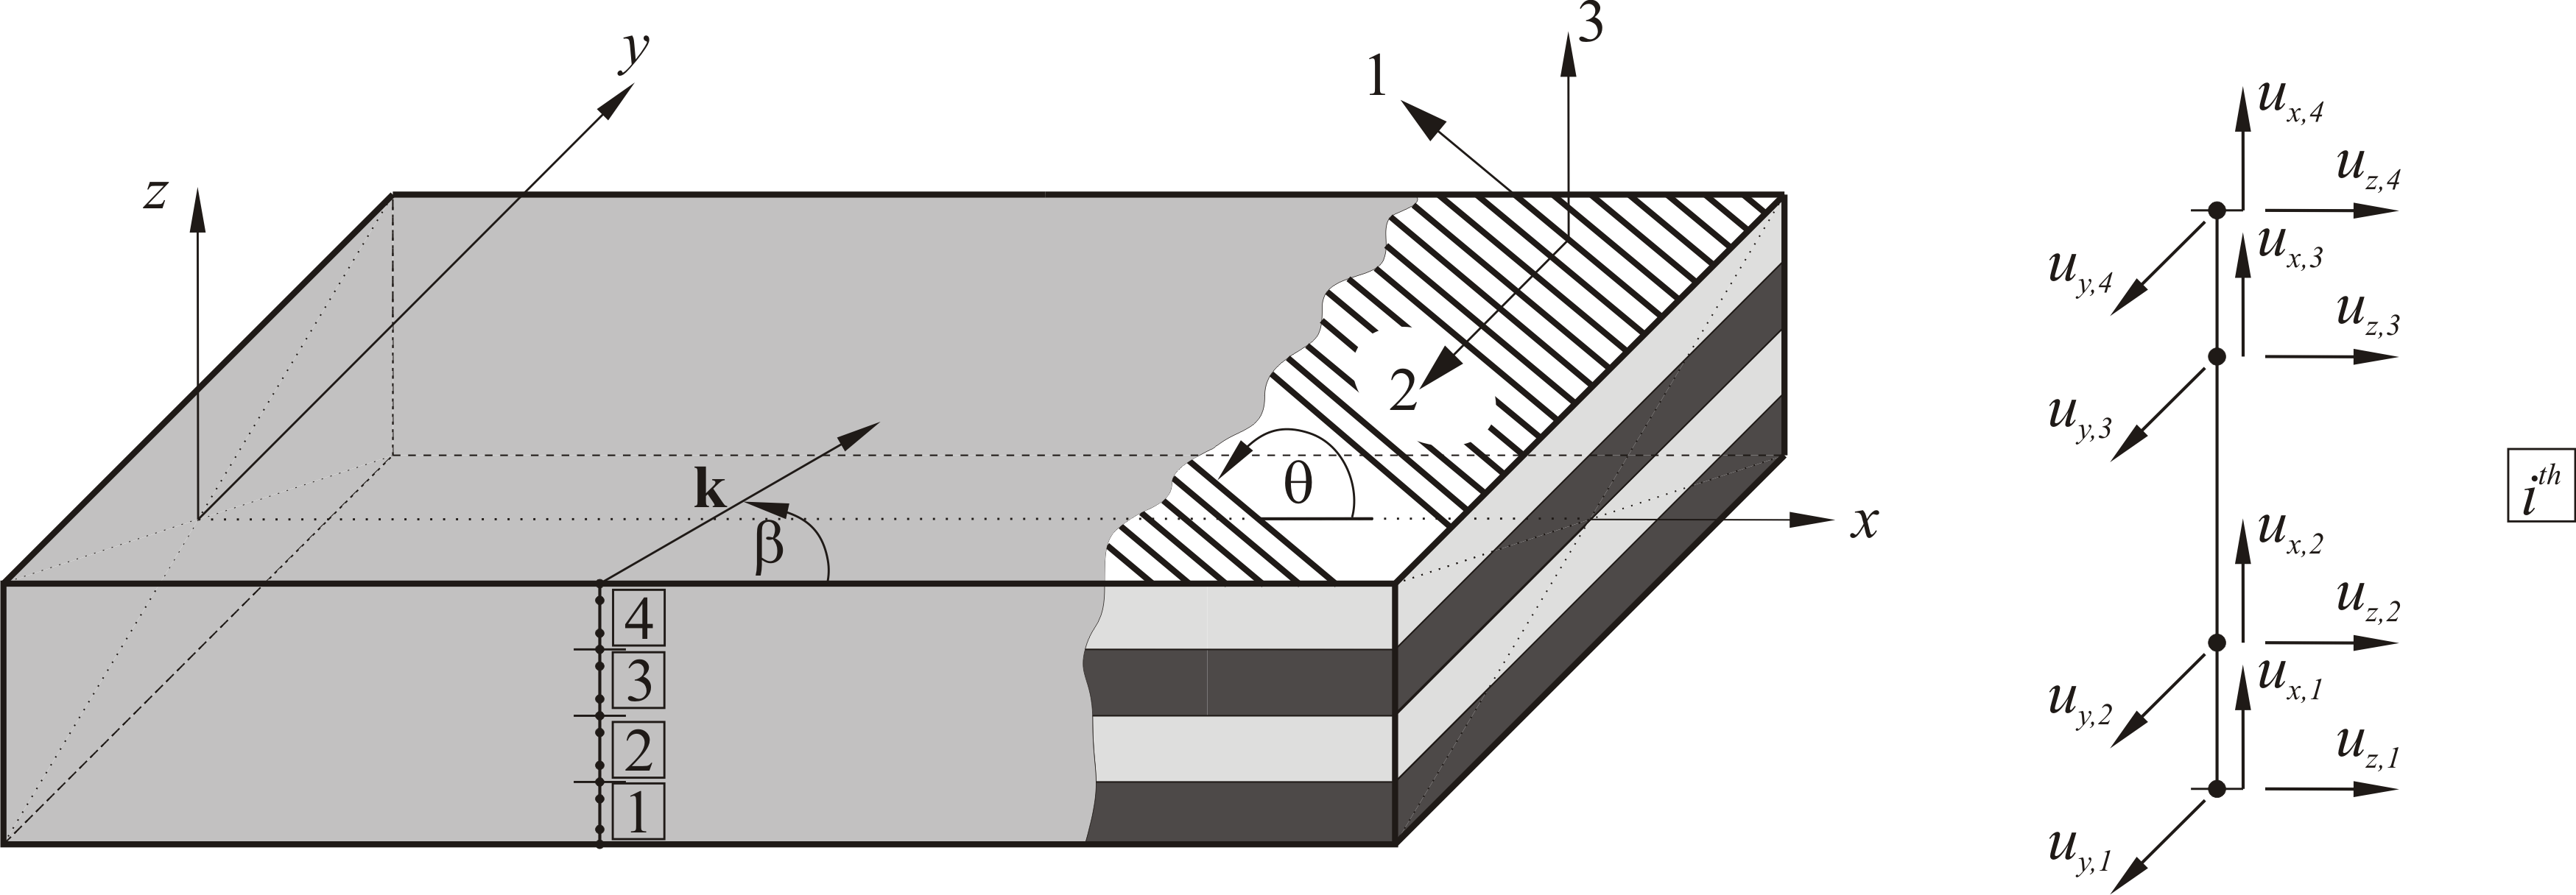
\includegraphics[width=\textwidth]{layered_composite_SASE4.png}
	%\includegraphics{layered_composite_SASE.png}	
	\caption{SASE model of wave propagation along with degrees of freedom of a one-dimensional four-node spectral element.}
	\label{fig:layered_composite_SASE}
\end{figure}
	
Additionally, according to the concept proposed by Taupin et~al.~\cite{Taupin2011}, equations for dispersion curves are derived so that the solution can be obtained for an arbitrary angle of propagation $\beta$ shown in Fig.~\ref{fig:layered_composite_SASE}. 
The wave propagation direction corresponds to the wavevector $\vect{k}$ defined as:
	
\begin{equation}
	\vect{k} = k \cos (\beta)\hat{ \vect{x}} + k \sin (\beta) \hat{\vect{y}},
	\label{eq:wavevector}
\end{equation}
where \(\hat{ \vect{x}}\) and \(\hat{\vect{y}}\) are unit vectors. 	
The general wave equation has a form of eigenvalue problem:

\begin{equation}
	\left[\matr{A} - \omega^2\matr{M} \right] \vect{U} =0,
	\label{eq:eig_dispersion}
\end{equation}
where $\omega$ is the angular frequency, $\matr{M}$ is the mass matrix, $\matr{U}$ is the nodal displacement vector, and the matrix $\matr{A}$ can be defined as:
\begin{equation}
	\begin{aligned}
	\matr{A} & =  k^2\left(s^2 \,\matr{K}_{22} + c^2\, \matr{K}_{33} - c s\, \matr{K}_{23} - c s\, \matr{K}_{32}\right) \\
	& + i k\, \matr{T}^T\left(-c\, \matr{K}_{13} - s\, \matr{K}_{21} + s\, \matr{K}_{12} + c\, \matr{K}_{31}\right) \matr{T} +\matr{K}_{11},
	\end{aligned}
	\label{eq:dispersion}
\end{equation}
where  $s = \sin(\beta)$, $c = \cos(\beta)$, $i = \sqrt{-1}$, and $\beta$ is the angle of guided wave propagation. 
The transformation matrix $\matr{T}$ is diagonal and it is introduced in order to eliminate imaginary elements from Eq.~(\ref{eq:dispersion}) (see~\cite{Bartoli2006} for more details). 
It should be noted that the system of equations~(\ref{eq:eig_dispersion}) explicitly depends on the angle $\beta$. 
Predicting the anisotropic behaviour of guided wave properties makes it necessary to loop over $\beta$ for each direction considered.
	
Stiffness matrices $\matr{K}_{mn}$ from Eq.~(\ref{eq:dispersion}) depend on elastic constants of composite laminate $\matr{C}$ and relations between displacements and strains. 
The definitions of these matrices on an elemental level are:
\begin{equation}
	\matr{K}_{mn}^e= \int \limits_{(e)} \matr{B}_m^{T} \matr{C}_{\theta}^e \, \matr{B}_n\, \ud z, 
	\label{eq:stiffness_matrix_e}
\end{equation}
where \(\matr{C}_{\theta}\) is the elastic tensor at spectral element (e) transformed by an angle \(\theta\) according to a stacking sequence: $ \matr{C}_{\theta}= \matr{R}_1(\theta) \,\matr{C} \,\matr{R}_2^{-1}(\theta)$; \(\matr{B}\) is the matrix relating displacements and strains.
More detailed derivation can be found in~\cite{Kudela2020}. 

The matrix of elastic constants of an orthotropic linear elastic material can be written as:
\begin{equation}
	\matr{C} = \left[\begin{array}{cccccc} C_{11} & C_{12}& C_{13} & 0&0&0\\[2pt]
		C_{12}& C_{22} & C_{23}& 0&0&0\\[2pt]
		C_{13}&C_{23}&C_{33}&0&0&0\\[2pt]
		0& 0 &0&C_{44}& 0&0\\[2pt]
		0&0&0&0&C_{55}&0\\[2pt]
		0&0&0&0&0&C_{66}
	\end{array}\right]. 
	\label{eq:elastic_constatns}
\end{equation} 
It means that there are 9 independent coefficients which should be determined by using an inverse method. 
	
Equation~(\ref{eq:eig_dispersion}) can be solved numerically in two ways:
\begin{itemize}
	\item as a standard eigenvalue problem $\omega (k)$ (assuming given real values of wavenumbers $k$),
	\item as a second-order polynomial eigenvalue problem $k(\omega)$ for given frequencies $\omega$.
\end{itemize}
In the former case, the standard eigenvalue problem has a form:
\begin{equation}
	\left[\matr{A} - \omega^2\matr{M} \right]_{m} \vect{U} =0,
	\label{eq:eig_standard}
\end{equation}
in which the number of equations is $m$.
In the later case, the solution consists of recasting Eq.~(\ref{eq:eig_standard}) to a first-order eigensystem by doubling its algebraic size:
\begin{equation}
	\left[\hat{\matr{A}} - k \hat{\matr{D}} \right]_{2m} \hat{\vect{Q}} =0,
	\label{eq:eig_poly}
\end{equation}  
where
\begin{equation*}
	\hat{\vect{Q}} =\left[\begin{array}{c} 
		\vect{U}\\
		k \vect{U}
	\end{array} \right],
\end{equation*}
\begin{flalign*}
	&\hat{\matr{A}} =\left[\begin{array}{cc} 
		0 & \matr{K}_{11} - \omega^2 \matr{M}\\
		\matr{K}_{11} - \omega^2 \matr{M} & -i \left( c	\, \matr{K}_{13} - s\, \matr{K}_{12}  + s\, \matr{K}_{21} - c \, \matr{K}_{31}   \right)
	\end{array} \right],   \\
	&\hat{\matr{D}} =\left[\begin{array}{cc} 
		\matr{K}_{11} - \omega^2 \matr{M} & 0\\
		0& - \left( s^2 \, \matr{K}_{22} + c^2 \,  \matr{K}_{33}  -s c \,  \matr{K}_{23}  -sc \, \matr{K}_{32}  \right)
	\end{array} \right].
\end{flalign*}
The obtained wavenumbers are then of a complex character. 
It provides information about both the wave dispersion (real part of the wavenumbers) and the attenuation of the waves (imaginary part of the wave numbers). 
Unfortunately, solving a second‐order polynomial eigenvalue problem is about 10 times more costly than solving a standard eigenvalue problem. 

Linear frequencies $f=\omega/2 \pi$ will be used in the next sections instead of angular frequencies $\omega$ for easier interpretation of figures.
%%%%%%%%%%%%%%%%%%%%%%%%%%%%%%%%%%%%%%%%%%%%%%%%%%%%%%%%%%%%%%%%%%%%%%%%%%%%%%%%
\section{Strategies for the determination of material properties \label{sec:strategies}}
%%%%%%%%%%%%%%%%%%%%%%%%%%%%%%%%%%%%%%%%%%%%%%%%%%%%%%%%%%%%%%%%%%%%%%%%%%%%%%%%
Dispersion curves calculated numerically must be accompanied by an experimental counterpart to build an appropriate objective function. 
In this paper, we consider guided waves acquired at a dense grid of points on the surface of a plate which forms full wavefield data set. 

Full wavefield data set can be acquired by scanning laser Doppler vibrometer (SLDV).
The data set is a 3D matrix representing spatial dimensions $x$, $y$ and the time $t$. 
Three-dimensional Fourier transform leads to the wavenumber-wavenumber-frequency representation  in the Cartesian coordinate system ($k_x$, $k_y$, $f$) or the wavenumber-angle-frequency representation in the cylindrical coordinate system ($k$, $\beta$, $f$).

Three strategies can be applied:
\begin{itemize}
	\item utilise data set at selected angle slices,
	\item utilise data set at selected frequency slices,
	\item use a mixed approach (not considered here).
\end{itemize}
%%%%%%%%%%%%%%%%%%%%%%%%%%%%%%%%%%%%%%%%%%%%%%%%%%%%%%%%%%%%%%%%%%%%%%%%%%%%%%%%
\subsection{Selected angle slices}
%%%%%%%%%%%%%%%%%%%%%%%%%%%%%%%%%%%%%%%%%%%%%%%%%%%%%%%%%%%%%%%%%%%%%%%%%%%%%%%%
The slices of the wavenumber-wavenumber-frequency data at selected wave propagation angles ($\beta=30^{\circ}$, $\beta=90^{\circ}$) are presented in Fig.~\ref{fig:angle_slice}. 
The slices reveal patterns which represent characteristic dispersion curves. 
Corresponding numerical dispersion curves can be computed quite fast by the semi-analytic method by swept over real wavenumber range.
Equation~(\ref{eq:eig_standard}) is used in this strategy.
The following wave propagation angles were considered in this paper: 0$^{\circ}$, 15$^{\circ}$, 30$^{\circ}$, 45$^{\circ}$, 60$^{\circ}$, 75$^{\circ}$ and 90$^{\circ}$.
\begin{figure} [h!]
	\centering
	\includegraphics{figure2.png}	
	\caption{Experimental wavenumber-wavenumber-frequency data sliced at chosen angles ($\beta=30^{\circ}$ and $\beta=90^{\circ}$).}
	\label{fig:angle_slice}
\end{figure}
%%%%%%%%%%%%%%%%%%%%%%%%%%%%%%%%%%%%%%%%%%%%%%%%%%%%%%%%%%%%%%%%%%%%%%%%%%%%%%%%
\subsection{Selected frequency slices}
%%%%%%%%%%%%%%%%%%%%%%%%%%%%%%%%%%%%%%%%%%%%%%%%%%%%%%%%%%%%%%%%%%%%%%%%%%%%%%%%
The data slices at frequencies 98.94 kHz and 349.43 kHz are shown in Fig.~\ref{fig:freq_slice}. 
The elliptic-like pattern of wavenumbers is visible (wavenumber surface).
In this case Eq.~(\ref{eq:eig_poly}) is more appropriate for calculation of equivalent numerical wavenumber profiles but it requires longer computation time as mentioned before.
The following frequency slices were considered in this paper: 48.85, 98.94, 149.04, 199.14, 249.24, 299.33 and 349.43~kHz giving the same number of slices as in the case of angle slices.
\begin{figure} [h!]
	\centering
	\includegraphics{figure3.png}	
	\caption{Experimental wavenumber-wavenumber-frequency data sliced at chosen frequencies (98.94 kHz and 349.43 kHz).}
	\label{fig:freq_slice}
\end{figure}
%%%%%%%%%%%%%%%%%%%%%%%%%%%%%%%%%%%%%%%%%%%%%%%%%%%%%%%%%%%%%%%%%%%%%%%%%%%%%%%%
\subsection{Objective function}
%%%%%%%%%%%%%%%%%%%%%%%%%%%%%%%%%%%%%%%%%%%%%%%%%%%%%%%%%%%%%%%%%%%%%%%%%%%%%%%%
The objective function consists of two parts: experimental which is in the form of an image and semi-analytical which is in the form of points which forms dispersion curves (or wavenumber profiles) calculated for the given elastic constants $C_{11}$, $C_{12}$, $C_{13}$, $C_{22}$, $C_{23}$, $C_{33}$, $C_{44}$, $C_{55}$ and $C_{66}$.
The semi-analytical dispersion characteristics (dispersion curves or wavenumber profiles) are converted to a binary image of the same resolution as in the experiment. 
In this way, we have experimental images and semi-analytical images of dispersion characteristics at selected angles of propagation. 
Semi-analytical images are used as filter masks for experimental images.
If dispersion curves from the SASE model align well with high values of experimental images, it leads to high values in the filtered image and vice versa.
Sum over pixel values of the resultant image is used as an objective function (see \cite{Kudela2020} for more details).
The objective function depending on optimisation strategy can be written as:
\begin{itemize}
	\item angle slice
\begin{equation}
	F=\min \frac{(-1)}{n_k \, n_f} \cdot \sum_{\beta} \sum_{i=1}^{n_k} \sum_{j=1}^{n_f} (D_{\beta}^{SASE})_{ij} \, \cdot (D_{\beta}^{EXP})_{ij},
	\label{eq:obj_fun_beta}
\end{equation}
where \(n_k\) is the number of wavenumber points and \(n_f\) is the number of frequency points, $\matr{D}_{\beta}^{SASE}$ is the binary image of dispersion curves calculated by the SASE model for the angle $\beta$ and $\matr{D}_{\beta}^{EXP}$ is the experimental image of the wavenumber-wavenumber-frequency data sliced at angle $\beta$.

\item frequency slice

\begin{equation}
	F=\min \frac{(-1)}{n_k \, n_{\beta}} \cdot \sum_{f} \sum_{i=1}^{n_k} \sum_{j=1}^{n_{\beta}} (D_{f}^{SASE})_{ij} \, \cdot (D_{f}^{EXP})_{ij},
	\label{eq:obj_fun_freq}
\end{equation}
where \(n_k\) is the number of wavenumber points and \(n_{\beta}\) is the number of angles, $\matr{D}_{f}^{SASE}$ is the binary image of wavenumber profiles calculated by the SASE model for the selected frequency $f$ and $\matr{D}_{f}^{EXP}$ is the experimental image of the wavenumber-wavenumber-frequency data sliced at frequency $f$.
\end{itemize}
%%%%%%%%%%%%%%%%%%%%%%%%%%%%%%%%%%%%%%%%%%%%%%%%%%%%%%%%%%%%%%%%%%%%%%%%%%%%%%%%
\subsection{Genetic algorithm parameters}
%%%%%%%%%%%%%%%%%%%%%%%%%%%%%%%%%%%%%%%%%%%%%%%%%%%%%%%%%%%%%%%%%%%%%%%%%%%%%%%%
The Sheffield Genetic Algorithm Toolbox for Matlab developed at the Department of Automatic Control and Systems Engineering at The University of Sheffield was used for the optimisation~\cite{Chipperfield1994}.
The genetic algorithm was used as an optimisation procedure due to the complex nature of the problem and form of the objective function. 
The objective function is non-differentiable, hence gradient methods cannot be applied. 

It should be noted that the genetic algorithm can stuck in local minima causing unwanted premature convergence. 
The mutation rate of 0.05 along with random offspring generation every 100-th generation was employed to alleviate the problem.

The remaining genetic algorithm parameters were as follows: the number of individuals 100, the maximum number of generations 800, generation gap 0.7, precision 9 bits, crossover rate 0.7,  random offspring generation rate 0.1.
%%%%%%%%%%%%%%%%%%%%%%%%%%%%%%%%%%%%%%%%%%%%%%%%%%%%%%%%%%%%%%%%%%%%%%%%%%%%%%%% 
\section{Guided wave modelling improvement through identification of elastic constants of unidirectional CFRP \label{sec:modelling_improvement}} 
%%%%%%%%%%%%%%%%%%%%%%%%%%%%%%%%%%%%%%%%%%%%%%%%%%%%%%%%%%%%%%%%%%%%%%%%%%%%%%%%
\subsection{Specimen}
The investigated specimen had dimensions 1200 $\times$ 1200 mm and was made out of carbon fibre-reinforced polymer (CFRP). 
The average thickness was 2.85 mm.
The total weight of the specimen was 6460 g, hence, based on the volume of the specimen, the density is about~1574.1~kg/m\textsuperscript{3}.
The specimen was composed of 40 layers of unidirectional prepregs stacked in one direction (90 degrees). 
NTPT thin prepregs 736LT 75~g/m$^2$ by North Thin Ply Technology and epoxy resin MP503Z-HT by Impregnatex Compositi were used for fabrication of the specimen.

The material properties of the specimen are given in Table~\ref{tab:mat_prop_uni}. 
It should be noted that only a few parameters are available in the specification delivered by the manufacturer. 
Other parameters were assumed as indicated in Table~\ref{tab:mat_prop_uni}.

\begin{table}[h]
	\renewcommand{\arraystretch}{1.3}
	\centering \footnotesize
	\caption{Material properties of unidirectional CFRP.}
	\begin{tabular}{lc} 
		\toprule
		Property & Value \\
		\midrule
		Epoxy density [kg/m\textsuperscript{3}]& 1150-1250\textsuperscript{1,3} \\ 
		Fibres density [kg/m\textsuperscript{3}]& 1800\textsuperscript{1}\\ 
		Young’s modulus of epoxy resin [GPa] & 3.43\textsuperscript{2}\\
		Young’s modulus of carbon fibres [GPa] & 230\textsuperscript{1}\\
		Poisson’s ratio of epoxy resin & 0.26\textsuperscript{2}\\
		Poisson’s ratio of carbon fibres & 0.20\textsuperscript{2} \\
		Volume fraction of reinforcing fibres & 0.552\textsuperscript{1}\\
		\bottomrule 
		\textsuperscript{1}Provided by manufacturer &\\
		\textsuperscript{2}Assumed &\\
		\textsuperscript{3}Assumed 1200 [kg/m\textsuperscript{3}]&\\
	\end{tabular} 
	\label{tab:mat_prop_uni}
\end{table}

%%%%%%%%%%%%%%%%%%%%%%%%%%%%%%%%%%%%%%%%%%%%%%%%%%%%%%%%%%%%%%%%%%%%%%%%%%%%%%%%
\subsection{Experimental measurements \label{sec:SLDV}}
%%%%%%%%%%%%%%%%%%%%%%%%%%%%%%%%%%%%%%%%%%%%%%%%%%%%%%%%%%%%%%%%%%%%%%%%%%%%%%%%
% laser vibrometer mesurements
Lamb waves were excited by a piezoelectric disk (PZT) of diameter 10 mm attached to the back surface of the specimen. 
Chirp signal with the frequency range 0-500 kHz lasting 200 $\mu$s was generated every 10 ms and applied to the PZT element through the signal amplifier.
The specimen central area of 455 $\times$ 455 mm was measured in 499 $\times$ 499 points using SLDV (Polytec PSV-400). 
In every measurement point, 2048 time samples were registered with a sampling frequency of 1.28 MHz. The measurements were taken 20 times in every grid point and averaged to improve the signal to noise ratio.
The measurement results were stored as a 3D matrix of size 499 $\times$ 499 $\times$ 2048 points. 
Median filtering was applied to remove noise in spatial images. Next 3D Fourier transform was applied. 
The resulting matrix was used for the determination of elastic constants.

Additional measurements were taken to validate the SEM model. 
The same setup was used but instead of a chirp signal, Hann windowed signal was applied for excitation at carrier frequencies 16.5 kHz, 50 kHz and 100 kHz. 
Five cycles in signals were used for each case. 
Moreover, measurements were taken only in one-quarter of the specimen at a grid of 491 $\times$ 491 points.
%%%%%%%%%%%%%%%%%%%%%%%%%%%%%%%%%%%%%%%%%%%%%%%%%%%%%%%%%%%%%%%%%%%%%%%%%%%%%%%%
\subsection{Data processing}
%%%%%%%%%%%%%%%%%%%%%%%%%%%%%%%%%%%%%%%%%%%%%%%%%%%%%%%%%%%%%%%%%%%%%%%%%%%%%%%%
Three-dimensional Fourier Transform was applied to the full wavefield data in the space-time domain ($x$, $y$, $t$). 
Next, 3D matrix was transformed from ($k_x$, $k_y$, $\omega$) coordinates to cylindrical coordinates ($k$, $\beta$, $f$). 
Interpolation was employed to obtain images $\matr{D}_{\beta}^{EXP}$ representing dispersion curves at selected angles $\beta = 0^{\circ} \ldots 90^{\circ}$ with the step of $15^{\circ}$. 
The size of the interpolated matrix $\matr{D}_{\beta}^{EXP}$ in the current approach was $n_k=512$ $\times$ $n_f= 512$. 
The result of this operation for selected angle slices is presented in Fig.~\ref{fig:angle_slice}. 

Similarly, interpolation was employed to obtain images $\matr{D}_{f}^{EXP}$ representing wavenumber surfaces at frequencies 48.85, 98.94, 149.04, 199.14, 249.24, 299.33 and 349.43~kHz.
The size of the interpolated matrix $\matr{D}_{f}^{EXP}$ in the current approach was $n_k=512$ $\times$ $n_{\beta}= 512$.
The result of this operation for selected frequency slices is presented in Fig.~\ref{fig:freq_slice}.
%%%%%%%%%%%%%%%%%%%%%%%%%%%%%%%%%%%%%%%%%%%%%%%%%%%%%%%%%%%%%%%%%%%%%%%%%%%%%%%%
\subsection{Determination of elastic constants}
%%%%%%%%%%%%%%%%%%%%%%%%%%%%%%%%%%%%%%%%%%%%%%%%%%%%%%%%%%%%%%%%%%%%%%%%%%%%%%%%
Two approaches were investigated: (i) the rule of mixtures followed by homogenisation based on material properties given in Table~\ref{tab:mat_prop_uni}, (ii) determination of elastic constants through the optimisation process described in section~\ref{sec:strategies}. 
The results of the rule of mixtures followed by homogenisation process are given in the second column of Table~\ref{tab:mat_prop_identified}.
The results of inversion by using $\beta$-slicing method and $f$-slicing method are given in the third and fourth column of Table~\ref{tab:mat_prop_identified}, respectively.
\begin{table}[h]
	\renewcommand{\arraystretch}{1.3}
	\centering \footnotesize
	\caption{Elastic material properties (Voigt notation).}
	\begin{tabular}{crrr} 
		\toprule
		Property & \multirow{2}{*}{Homogenised} & \multicolumn{2}{c}{Optimised}\\
		\cmidrule(lr){3-4}
		$\left[\textrm{GPa}\right]$ &  & $\beta$-slicing & $f$-slicing \\ 
		\midrule 
		$C_{11}$ & 130.11 & 138.67 & 138.24 \\ 
		$C_{12}$ & 3.56   & 5.72   & 7.65\\ 
		$C_{13}$ & 3.56   & 6.53   & 7.85\\
		$C_{22}$ & 12.31  & 12.36  & 13.84\\
		$C_{23}$ & 3.36   & 5.99  & 8.00\\
		$C_{33}$ & 12.31  & 11.80 & 14.38\\
		$C_{44}$ & 4.48   & 3.12  & 3.07\\
		$C_{55}$ & 4.51   & 5.11  & 5.11\\
		$C_{66}$ & 4.51   & 4.89  & 4.99 \\
		\bottomrule
	\end{tabular} 
	\label{tab:mat_prop_identified}
\end{table}
It can be noticed that optimised elastic properties given in Table~\ref{tab:mat_prop_identified} are significantly different than elastic constants estimated through homogenisation. 
The differences are as large as around 6\% for $C_{11}$ and up to 45\% for $C_{13}$ elastic constant.
These differences also contribute to differences in dispersion curves. 
Comparison of dispersion curves calculated by SASE method for homogenised material properties with dispersion curves calculated for optimised material properties is given in Fig.~\ref{fig:homog_opt}. 
White dispersion curves are overlaid on experimental images. 
Red and yellow colours on experimental images resemble dispersion curves where on the horizontal axis is the frequency $f$ and on the vertical axis is the wavenumber $k$. 

\begin{figure} [h!]
	\centering
	\begin{subfigure}[b]{0.47\textwidth}
		\centering
		\includegraphics[]{figure4a.png}
		\caption{SASE (homogenised) vs experimental; $\beta=0^{\circ}$}
		\label{fig:dispersion0deg_homog}
	\end{subfigure}
	\hfill
	\begin{subfigure}[b]{0.47\textwidth}
		\centering
		\includegraphics[]{figure4b.png}
		\caption{SASE (optimised) vs experimental; $\beta=0^{\circ}$}
		\label{fig:dispersion0deg_opt}
	\end{subfigure}
	\hfill
	\begin{subfigure}[b]{0.47\textwidth}
		\centering
		\includegraphics[]{figure4c.png}
		\caption{SASE (homogenised) vs experimental; $\beta=45^{\circ}$}
		\label{fig:dispersion45deg_homog}
	\end{subfigure}
	\hfill
	\begin{subfigure}[b]{0.47\textwidth}
		\centering
		\includegraphics[]{figure4d.png}
		\caption{SASE (optimised) vs experimental; $\beta=45^{\circ}$}
		\label{fig:dispersion45deg_opt}
	\end{subfigure}
	\hfill
	\begin{subfigure}[b]{0.47\textwidth}
		\centering
		\includegraphics[]{figure4e.png}
		\caption{SASE (homogenised) vs experimental; $\beta=60^{\circ}$}
		\label{fig:dispersion60deg_homog}
	\end{subfigure}
	\hfill
	\begin{subfigure}[b]{0.47\textwidth}
		\centering
		\includegraphics[]{figure4f.png}
		\caption{SASE (optimised) vs experimental; $\beta=60^{\circ}$}
		\label{fig:dispersion60deg_opt}
	\end{subfigure}
	\caption{Comparison of dispersion curves calculated by SASE method for homogenised material properties (left) with dispersion curves calculated for optimised material properties (right). White dispersion curves are overlaid on experimental images.}
	\label{fig:homog_opt}
\end{figure}

SASE curves calculated for the homogenised material properties are significantly overestimated at angle 0\(^{\circ}\) (in this case perpendicular to fibres) and slightly underestimated at angle 90° (parallel to fibres). 
The best fit is at about 45\(^{\circ}\). 
In contrast, SASE curves calculated for optimised material properties almost perfectly matches the red and yellow spots on experimental images. 
The objective function value $F$ is 97.11 for a homogenised case and 16.78 for the optimised case, respectively. 
In other words, the fitness of dispersion curves is much better for the latter case (the lower $F$ means better fitness).

It is worthy to note, that $f$-slicing method slightly better resembles some properties of the unidirectionally reinforced composite.
In such material, it is expected that shear related constants $C_{55}=C_{66}$ and extension-extension coupling constants related to the Poisson effect $C_{12}=C_{13}$.
It could be attributed to the larger number of angle points $n_{\beta}=512$ contributing to the objective function given by Eq.~{\ref{eq:obj_fun_freq}} in comparison to $\beta=7$ in Eq.~(\ref{eq:obj_fun_beta}).

Again, excellent agreement is obtained between optimised SASE wavenumber profiles and experimental images. 
Such a comparison is presented in Fig.~\ref{fig:freq_slice_opt}.
It can be seen that the higher the frequency, the more Lamb wave modes are propagating simultaneously.
At the frequency 349.43~kHz five modes contribute to the objective function through five wavenumber profile curves.

Moreover, $k_y$ wavenumbers have lower values than $k_x$ wavenumbers.
Therefore, it can be deduced from the relationship $c_p= f / k$ that elastic waves propagate faster in the vertical direction, as expected, because of the vertical orientation of fibres.

\begin{figure} [h!]
	\centering
	\begin{subfigure}[b]{0.47\textwidth}
		\centering
		\includegraphics[]{figure5a.png}
		%\caption{}
		\label{fig:freq3_slice_opt}
	\end{subfigure}
	\hfill
	\begin{subfigure}[b]{0.47\textwidth}
		\centering
		\includegraphics[]{figure5b.png}
		%\caption{}
		\label{fig:freq4_slice_opt}
	\end{subfigure}
	\hfill
	\begin{subfigure}[b]{0.47\textwidth}
		\centering
		\includegraphics[]{figure5c.png}
		%\caption{}
		\label{fig:freq5_slice_opt}
	\end{subfigure}
	\hfill
	\begin{subfigure}[b]{0.47\textwidth}
		\centering
		\includegraphics[]{figure5d.png}
		%\caption{}
		\label{fig:freq7_slice_opt}
	\end{subfigure}
	\caption{Comparison of wavenumber profiles calculated by SASE method for optimised material properties (white curves) with experimental images.}
	\label{fig:freq_slice_opt}
\end{figure}
%%%%%%%%%%%%%%%%%%%%%%%%%%%%%%%%%%%%%%%%%%%%%%%%%%%%%%%%%%%%%%%%%%%%%%%%%%%%%%%%
\subsection{SEM model}
%%%%%%%%%%%%%%%%%%%%%%%%%%%%%%%%%%%%%%%%%%%%%%%%%%%%%%%%%%%%%%%%%%%%%%%%%%%%%%%%
The goal was to model as accurately as possible full wavefield of guided waves for the case of piezoelectric excitation at the centre of the plate. 
The same excitation frequencies, namely 16.5 kHz, 50 kHz and 100 kHz were considered as in the experiment. 
The time-domain spectral element method was used in which a shell model based on the first-order shear deformation theory is implemented~\cite{Kudela2020a}. 
In this model, the composite laminate is represented only by a mid-surface. Therefore, equivalent elastic properties must be calculated. 

Elastic constants estimated by both homogenisation as well as optimisation methods are given in Table~\ref{tab:mat_prop_identified}. 
It should be noted that in the shell model, the assumption is made that the strain in the thickness direction is zero. 
Therefore only 6 of 9 constants given in Table~\ref{tab:mat_prop_identified} are required in the SEM model.

It should be added that the unstructured mesh of the SEM model was generated by using Gmsh software~\cite{Geuzaine2009} rendering pzt disc at the centre where equivalent piezoelectric forces were applied. 
The mesh was tailored to the highest investigated carrier frequency to ensure at least 8 nodes per wavelength.

%%%%%%%%%%%%%%%%%%%%%%%%%%%%%%%%%%%%%%%%%%%%%%%%%%%%%%%%%%%%%%%%%%%%%%%%%%%%%%%%
\subsection{SEM model accuracy analysis}
%%%%%%%%%%%%%%%%%%%%%%%%%%%%%%%%%%%%%%%%%%%%%%%%%%%%%%%%%%%%%%%%%%%%%%%%%%%%%%%%
It should be underlined that the SASE model is used in the optimisation algorithm. 
It enables to use of one element per composite layer giving very accurate dispersion characteristics. The purpose of SEM model is different. 
It is used for full wavefield analysis and often analysis of the interaction of Lamb waves with defects. 
It requires a dense mesh of nodes. 
Since the representation of each layer of a composite laminate is prohibitive due to high computation cost, approximate theories are used. 
In the present approach, first-order shear deformation theory was applied. 
However, higher-order theories can be used as well (see~\cite{Ostachowicz2012}).

Since guided wave damage detection methods usually rely on fundamental Lamb wave modes, i.e. S0 and A0, accurate representation of these modes by the model is crucial.
We focus here on A0 mode analysis. 
In particular, transverse displacements are extracted from the SEM model and interpolated at the uniform grid of points so that the Fourier transform can be applied. 
Numerical full wavefield data sets calculated for the investigated carrier frequencies were processed by the 3D Fourier transform and next combined. 
Due to the fact, that Hann windowed signal with 5 cycles has some frequency bandwidth, the combined image gives a good representation of A0 mode dispersion curve as shown in Fig.~\ref{fig:homog_opt_num}. 
\begin{figure} [h!]
	\centering
	\begin{subfigure}[b]{0.47\textwidth}
		\centering
		\includegraphics[]{figure6a.png}
		%\caption{SASE (optim.) vs SEM (homog.); $\beta=0^{\circ}$}
		%\label{fig:dispersion0deg_homog_num}
	\end{subfigure}
	\hfill
	\begin{subfigure}[b]{0.47\textwidth}
		\centering
		\includegraphics[]{figure6b.png}
		%\caption{SASE (optim.) vs SEM (optim.); $\beta=0^{\circ}$}
		%\label{fig:dispersion0deg_opt_num}
	\end{subfigure}
	\hfill
	\begin{subfigure}[b]{0.47\textwidth}
		\centering
		\includegraphics[]{figure6c.png}
		%\caption{SASE (optim.) vs SEM (homog.); $\beta=45^{\circ}$}
		%\label{fig:dispersion45deg_homog_num}
	\end{subfigure}
	\hfill
	\begin{subfigure}[b]{0.47\textwidth}
		\centering
		\includegraphics[]{figure6d.png}
		%\caption{SASE (optim.) vs SEM (optim.); $\beta=45^{\circ}$}
		%\label{fig:dispersion45deg_opt_num}
	\end{subfigure}
	\hfill
	\begin{subfigure}[b]{0.47\textwidth}
		\centering
		\includegraphics[]{figure6e.png}
		%\caption{SASE (optimised) vs SEM (homog.); $\beta=60^{\circ}$}
		%\label{fig:dispersion60deg_homog_num}
	\end{subfigure}
	\hfill
	\begin{subfigure}[b]{0.47\textwidth}
		\centering
		\includegraphics[]{figure6f.png}
		%\caption{SASE (optim.) vs SEM (optim.); $\beta=60^{\circ}$}
		%\label{fig:dispersion60deg_opt_num}
	\end{subfigure}
	\caption{Comparison of A0 mode dispersion images calculated by the SEM model for the homogenised material properties (left) and optimised material properties (right). White A0 mode dispersion curves calculated by SASE model for optimised material properties are given as a reference. }
	\label{fig:homog_opt_num}
\end{figure}

Figure~\ref{fig:homog_opt_num} shows the comparison of A0 mode dispersion images calculated by the SEM model for the homogenised material properties and optimised material properties obtained by the $\beta$-slicing method as given in Table~\ref{tab:mat_prop_identified}. 
White A0 mode dispersion curves calculated by the SASE model for optimised material properties obtained by the $\beta$-slicing method are given as a reference. 
It is confirmed that homogenised material properties lead to significant error in dispersion curves which directly translate to errors in phase velocities given by relationship $c_p= f/k$.

It is important to note that despite low-order approximation of shell SEM, dispersion images match very well SASE dispersion curves (right column of Fig.~\ref{fig:homog_opt_num}). 
Only slight discrepancies at higher frequencies (100~kHz) are visible. 
These discrepancies are consistent for each investigated angle of propagation – wavenumbers are underestimated, therefore phase velocities from SEM model are too high by about 0.7\%.
%%%%%%%%%%%%%%%%%%%%%%%%%%%%%%%%%%%%%%%%%%%%%%%%%%%%%%%%%%%%%%%%%%%%%%%%%%%%%%%%
\subsection{Full wavefield comparison}
%%%%%%%%%%%%%%%%%%%%%%%%%%%%%%%%%%%%%%%%%%%%%%%%%%%%%%%%%%%%%%%%%%%%%%%%%%%%%%%%
Another visualisation is shown in Fig.~\ref{fig:wavefield_comparison} to underline the importance of accurate modelling of guided waves velocity. 
A frame of propagating waves is selected at the time instance 0.5~ms. 

Reinforcing fibres are located vertically, hence wavefront is elongated in the vertical direction.
The image in Fig.~\ref{fig:wavefield_sem_homog} shows that the application of homogenised material properties causes that the A0 mode reaches the left edge too fast. 
In contrast, the application of optimised material properties results in a wave pattern (Fig.~\ref{fig:wavefield_sem_opt}) which is very similar to the experimental one (Fig.~\ref{fig:wavefield_exp}) except for wave crest amplitudes. 
The A0 mode calculated numerically based on elastic constants obtained by angle-slicing method reaches the left edge at the same time as in the experiment.
\begin{figure} [h!]
	\centering
	\begin{subfigure}[t]{0.32\textwidth}
		\centering
		\includegraphics[width=\textwidth]{figure7a.png}
		\caption{Numerical SEM (homog.)}
		\label{fig:wavefield_sem_homog}
	\end{subfigure}
	\hfill
	\begin{subfigure}[t]{0.32\textwidth}
		\centering
		\includegraphics[width=\textwidth]{figure7b.png}
		\caption{Numerical SEM (optim.)}
		\label{fig:wavefield_sem_opt}
	\end{subfigure}
	\hfill
	\begin{subfigure}[t]{0.32\textwidth}
		\centering
		\includegraphics[width=\textwidth]{figure7c.png}
		\caption{Experimental}
		\label{fig:wavefield_exp}
	\end{subfigure}
	\caption{Comparison of wavefields of propagating guided waves for the excitation frequency 50~kHz at the time instance 0.5 ms.}
	\label{fig:wavefield_comparison}
\end{figure}
\clearpage
%%%%%%%%%%%%%%%%%%%%%%%%%%%%%%%%%%%%%%%%%%%%%%%%%%%%%%%%%%%%%%%%%%%%%%%%%%%%%%%%
\section{Validation on quasi-isotropic CFRP plate\label{sec:validation}}
%%%%%%%%%%%%%%%%%%%%%%%%%%%%%%%%%%%%%%%%%%%%%%%%%%%%%%%%%%%%%%%%%%%%%%%%%%%%%%%%
It should be noted that despite an excellent agreement between numerical and experimental dispersion curves reported in section~\ref{sec:modelling_improvement}, the correctness of elastic tensor $\matr{C}$ is not entirely proven.
Therefore, additional effort was made to validate its correctness.
The validation was conducted based on Open Guided Waves (OGW) data set which is accompanied by material properties obtained by various test standards~\cite{Moll2019}.
OGW is an extendable online platform where high-quality and well-documented datasets for guided wave-based inspections are provided.
%%%%%%%%%%%%%%%%%%%%%%%%%%%%%%%%%%%%%%%%%%%%%%%%%%%%%%%%%%%%%%%%%%%%%%%%%%%%%%%%
\subsection{Specimen and material properties \label{sec:spec}}
%%%%%%%%%%%%%%%%%%%%%%%%%%%%%%%%%%%%%%%%%%%%%%%%%%%%%%%%%%%%%%%%%%%%%%%%%%%%%%%%
The benchmark structure used for validation was quasi-isotropic carbon-fibre-reinforced polymer (CFRP) plate with embedded piezoelectric transducers. 
The specimen was made of prepreg material Hexply\textsuperscript{\textregistered} M21/34\%/\-UD134/\-T700/\-300.
The layup was [45/0/-45/90/-45/0/45/90]\textsubscript{S}. 
CFRP plate had the dimensions of 500 mm \(\times\) 500 mm and a thickness of 2 mm 
(values provided by the manufacturer). 
The actual measured average thickness was 2.086 mm. 
The diameter of the piezoelectric transducers was 10 mm and the thickness 0.2 mm. 

The established material properties by various test standards for unidirectional Hexply material are given in Table~\ref{tab:mat_prop_Moll}. 

\begin{table}
	\renewcommand{\arraystretch}{1.3}
	\centering \footnotesize
	\caption{Material properties of unidirectional Hexply M21/34\%/UD134/T700/300.}
		\begin{tabular}{crclc} 
			\toprule
			Property &  \multicolumn{1}{c}{Value}  & Units & \multicolumn{1}{c}{Test standard} & Source \\
			\midrule
			$E_{11}$ & 125.5$\pm$ 2.4   & GPa & DIN EN ISO 527-5 & \cite{Moll2019} \\
			$E_{22}$ & 8.7$\pm$ 0.1     & GPa & DIN EN ISO 527-5 & \cite{Moll2019} \\
			$G_{12}$ & 4.135 $\pm$ 0.07 & GPa & EN ISO 14129 & \cite{Petersen2016} \\
			$\nu_{12}$ & 0.37$\pm$ 0.08 & -   & DIN EN ISO 527-5 & \cite{Moll2019} \\
			$\nu_{23}$ & 0.45$\pm$ 0.02 & -   & DIN EN ISO 527-5 & \cite{Moll2019} \\
			$\rho$ & 1571$\pm$ 2 & kg/m\textsuperscript{3}   & - & \cite{Moll2019} \\
			\bottomrule 
		\end{tabular} 
		\label{tab:mat_prop_Moll}
\end{table}
The matrix of elastic constants $\matr{C}$ was calculated based on the material properties given in Table~\ref{tab:mat_prop_Moll} and the formulas:
\begin{equation}
	\frac{\nu_{ij}}{E_{ii}}=\frac{\nu_{ji}}{E_{jj}},\quad i,j=1,2,3\quad i\ne j
	\label{eq:recalc}
\end{equation}
and 
\begin{equation}
	G_{23} = \frac{E_{22}}{2\,(1+\nu_{23})}.
	\label{eq:recalc2}
\end{equation}
Also, the aspect of propagation of uncertainties was taken into account.
The results are given in Table~\ref{tab:mat_prop_identified_Moll} and are labelled as "Reference".
%%%%%%%%%%%%%%%%%%%%%%%%%%%%%%%%%%%%%%%%%%%%%%%%%%%%%%%%%%%%%%%%%%%%%%%%%%%%%%%%
\subsection{Experimental measurements}
%%%%%%%%%%%%%%%%%%%%%%%%%%%%%%%%%%%%%%%%%%%%%%%%%%%%%%%%%%%%%%%%%%%%%%%%%%%%%%%%
Experimental full wavefield measurements by using SLDV were conducted in a similar manner as it was described in section~\ref{sec:SLDV}. 
However, only a quarter of the plate was considered for 3D Fourier transform.
It should be added that 0\(^{\circ}\) fibre orientation was along the vertical edge of the specimen.
%%%%%%%%%%%%%%%%%%%%%%%%%%%%%%%%%%%%%%%%%%%%%%%%%%%%%%%%%%%%%%%%%%%%%%%%%%%%%%%%
\subsection{Determination of elastic constants}
%%%%%%%%%%%%%%%%%%%%%%%%%%%%%%%%%%%%%%%%%%%%%%%%%%%%%%%%%%%%%%%%%%%%%%%%%%%%%%%%
The determined elastic constants are gathered in Table~\ref{tab:mat_prop_identified_Moll}.
The reference values are calculated based on OGW data as it was explained in section~\ref{sec:spec}.
It should be noted that reference elastic constants are characterised by high variability expressed by high values of standard deviation.
In the next column results obtained by $\beta$-slicing method are presented followed by standard deviations calculated based on 10 genetic algorithm runs.
Due to long computation time, only one genetic algorithm run was used to determine elastic constants by using $f$-slicing method.

The optimised $C_{11}$ elastic constants are slightly lower than reference values.
The optimised $C_{12}$ and $C_{13}$ elastic constants are up to 46\% greater than the reference values.
Similarly $C_{22}$ constant seems to be overestimated by about 32\% in comparison to the reference values.
Overall, it seems that the optimised elastic constants differs quite substantially from the reference values.
Nevertheless, the wavenumber profiles calculated by using optimised elastic constants better fit to the experimental data than the wavenumber profiles calculated by using reference elastic constants (see Fig.~\ref{fig:freq_slice_opt_Moll}).
This is especially visible at higher frequencies for larger values of wavenumbers.
The most outward white curve (corresponding to A0 Lamb wave mode) in Fig.~\ref{fig:freq_slice_opt_Moll} fit better to the experimental wavenumber map than magenta curve.
%However, neither of these curves fit perfectly to the experimental wavenumber map.
On the other hand, the wavenumber profiles corresponding to SH0 mode and S0 mode calculated for reference elastic constants and optimised elastic constants overlap.

It might mean that static test standards (see Table~\ref{tab:mat_prop_Moll}) along with formulas given by Eqs.~(\ref{eq:recalc})-(\ref{eq:recalc2}) are appropriate for lower frequency ranges and longer wavelengths.
But for high frequency problems such as Lamb wave propagation phenomenon, the alternative method for determination of elastic constants should be applied.
In this context, optimised elastic constants obtained by the proposed methods should be considered valid.
\begin{table}[h]
	\renewcommand{\arraystretch}{1.3}
	\centering \footnotesize
	\caption{Elastic material properties of Hexply M21/34\%/UD134/T700/300 CFRP (Voigt notation).}
	\begin{tabular}{crrr} 
		\toprule
		Property & \multicolumn{1}{c}{Reference} & \multicolumn{2}{c}{Optimised}\\
		\cmidrule(lr){3-4}
		$\left[\textrm{GPa}\right]$ & \multicolumn{1}{c}{\cite{Moll2019}} & $\beta$-slicing & $f$-slicing \\ 
		\midrule 
		$C_{11}$ & 129.99$\pm$12.22  & 119.59$\pm$5.12 & 119.19 \\ 
		$C_{12}$ &   6.06$\pm$ 1.08  &   8.87$\pm$0.09 &   8.91\\ 
		$C_{13}$ &   6.06$\pm$ 1.08  &   7.47$\pm$1.39 &   8.59\\
		$C_{22}$ &  11.19$\pm$ 3.51  &  16.47$\pm$0.04 &  14.78\\
		$C_{23}$ &   5.19$\pm$ 0.42  &   2.51$\pm$0.02 &   5.27\\
		$C_{33}$ &  11.19$\pm$ 3.51  &   5.74$\pm$0.19 &   9.03\\
		$C_{44}$ &   3.00$\pm$ 0.14  &   2.95$\pm$0.12 &   3.45\\
		$C_{55}$ &   4.13$\pm$ 0.07  &   5.85$\pm$0.49 &   5.44\\
		$C_{66}$ &   4.13$\pm$ 0.07  &   4.46$\pm$0.95 &   5.37 \\
		\bottomrule
	\end{tabular} 
	\label{tab:mat_prop_identified_Moll}
\end{table}

\begin{figure} [h!]
	\centering
	\begin{subfigure}[b]{0.47\textwidth}
		\centering
		\includegraphics[]{figure8a.png}
		\caption{}
		\label{fig:freq3_opt_Moll}
	\end{subfigure}
	\hfill
	\begin{subfigure}[b]{0.47\textwidth}
		\centering
		\includegraphics[]{figure8b.png}
		%\caption{}
		\label{fig:freq4_opt_Moll}
	\end{subfigure}
	\hfill
	\begin{subfigure}[b]{0.47\textwidth}
		\centering
		\includegraphics[]{figure8c.png}
		%\caption{}
		\label{fig:freq5_opt_Moll}
	\end{subfigure}
	\hfill
	\begin{subfigure}[b]{0.47\textwidth}
		\centering
		\includegraphics[]{figure8d.png}
		%\caption{}
		\label{fig:freq7_opt_Moll}
	\end{subfigure}
	\caption{Comparison of the wavenumber profiles calculated by SASE method for optimised material properties (white curves) and reference case based on OGW (magenta curves) with experimental images.}
	\label{fig:freq_slice_opt_Moll}
\end{figure}
\clearpage
%%%%%%%%%%%%%%%%%%%%%%%%%%%%%%%%%%%%%%%%%%%%%%%%%%%%%%%%%%%%%%%%%%%%%%%%%%%%%%%%
\section{Conclusions}
%%%%%%%%%%%%%%%%%%%%%%%%%%%%%%%%%%%%%%%%%%%%%%%%%%%%%%%%%%%%%%%%%%%%%%%%%%%%%%%%
We presented the guided wave propagation framework which consists of two steps. 
In the first step, 9 elastic constants of the carbon-fibre-reinforced composite are determined through the optimisation process. 
Genetic algorithm is employed for optimisation of difference between dispersion curves obtained experimentally and dispersion curves calculated numerically by SASE method.
In the second step, full wavefield simulations were performed by using the time domain SEM. 
It has been shown that very good agreement can be obtained between SEM and experiment if optimised elastic constants are used. 
Such an approach is much preferred in comparison to homogenisation techniques because it leads to much lower errors in guided wave velocities.

The validation of the correctness of the proposed optimisation method was performed based on the OGW data set.
It has been found that the optimised elastic constants differs quite substantially from the reference values. 
But the wavenumber profiles calculated by using optimised elastic constants fit better the experimental data than the wavenumber profiles calculated by using reference elastic constants.
It might be attributed to the fact that the proposed approach of elastic constant determination is more suitable for high-frequency problems such as Lamb wave propagation phenomenon than static test standards.

In summary, the current implementation of the SEM, in which elastic constants are determined first, is very well suited for model-based structural health monitoring. 
It is because modelled Lamb wave velocities and wavefront profiles are very close to experimental data obtained by SLDV. 

Analysis of improvement in the wave attenuation modelling and wave crest amplitude distribution through optimisation is a task which is planned in the future.

%%%%%%%%%%%%%%%%%%%%%%%%%%%%%%%%%%%%%%%%%%%%%%%%%%%%%%%%%%%%%%%%%%%%%%%%%%%%%%%%
\section*{Acknowledgement}
%%%%%%%%%%%%%%%%%%%%%%%%%%%%%%%%%%%%%%%%%%%%%%%%%%%%%%%%%%%%%%%%%%%%%%%%%%%%%%%%
The research was funded by the Polish National Science Center under grant agreement no 2018/29/B/ST8/00045. 
		
	%% If you have bibdatabase file and want bibtex to generate the
	%% bibitems, please use
	%%
	%%  \bibliographystyle{elsarticle-harv} 
	%%  \bibliography{<your bibdatabase>}
	
	%% else use the following coding to input the bibitems directly in the
	%% TeX file.
	%\section*{Reference}
    \bibliographystyle{num_order}
	\bibliography{2021-Identification-GA}{}

\end{document}


